\subsection{Question 1}

\begin{equation}
	\begin{aligned}
		RE &= |\frac{b-a}{b}|\\
		0.1 &= \frac{1}{2^5} + \frac{1}{2^6} + \frac{1}{2^8} + RE \\
		&= 0.1015625
	1\end{aligned}
\end{equation}

L'erreur est donc de $|\frac{0.1015625 - 0.1}{0.1}| = 0.015625$ soit une erreur de moins de 5 \%.

Rien que pour représenter la partie décimale, il faut donc 8 bits. Cela ne tiens pas compte ni du bit pour le signe ni des bits pour représenter la partie entière.

\subsection{Question 2}

\begin{equation}
	\begin{aligned}
		x &= [\underline{x}, \overline{x}]\\
		y &= [\underline{y}, \overline{y}]
	\end{aligned}
\end{equation}

On peut donc calculer la somme et le produit de $x$ et $y$ de cette manière :

\begin{equation}
	\begin{aligned}
		x + y &= [\underline{x} + \underline{y}, \overline{x} + \overline{y}]\\
		x \cdot y &= [\underline{x} \cdot \underline{y}, \overline{x} \cdot \overline{y}]
	\end{aligned}
\end{equation}

\subsection{Question 3}

\subsubsection{Point 1}

\paragraph{Très petit x}
Si $x_i \ll 0$, alors $e^x$ va devenir très petit. En effet, $e^{x} = \frac{1}{e^{|x|}}$ (pour $x$ négatif). $e^{|x|}$ sera donc grand et du coup $\frac{1}{e^{|x|}}$ sera très petit. On peut même dire que si $x$ est fortement négatif, $e^x$ tend vers 0. On obtiens alors $log(0+0+...+0) = log(0)$, ce qui est impossible. On aura donc une erreur lors de l'exécution de $log(0)$.

\paragraph{Très grand x}
Si $x_i \gg 0$, alors $e^x$ va devenir très grand, et on va très rapidement etteindra la capacité maximale et provoquer un $overflow$. On aura donc également une erreur, mais cette erreur aura lieu cette fois-ci dès le calcul de $e^x$.

\subsubsection{Point 2}

On peut remplacer chaque $x_i$ par $x_i-a+a$, où $a = max|\text{Valeur }x_i|$ :

\begin{equation}
	\begin{aligned}
		log(e^{a+x_i-a}+...+e^{a+x_i-a}) &= log (e^a(e^{x_i-a}+...+e^{x_i-a})\\
		&= log (e^a)+log(\sum e^{x_i-a})\\
		&= a+log(\sum e^{x_i-a})\\
	\end{aligned}
\end{equation}

\subsection{Question 4}

La méthode main contient deux variables, \texttt{start} et \texttt{end} qui déterminent les bornes où évaluer la fonction. La variable \texttt{pointsToCalculate} détermine le nombre de points à calculer. Les points seront répartis de manière uniforme entre \texttt{start} et \texttt{end}.

\code{littleclasses}{expo.java}

Et voici le graphique généré via gnuplot\footnote{\url{http://www.gnuplot.info}} avec comme paramètre \texttt{pointsToCalculate} à 100 :

\begin{figure}[H]
	\caption{\label{ex} Plot avec 100 points de calcul}
	\centering
	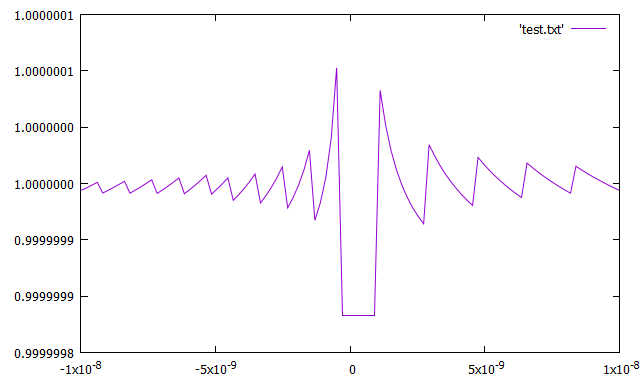
\includegraphics[scale = 0.61]{Figures/1_plot.png}
\end{figure}
